% Created by tikzDevice version 0.12.6 on 2025-08-19 18:43:19
% !TEX encoding = UTF-8 Unicode
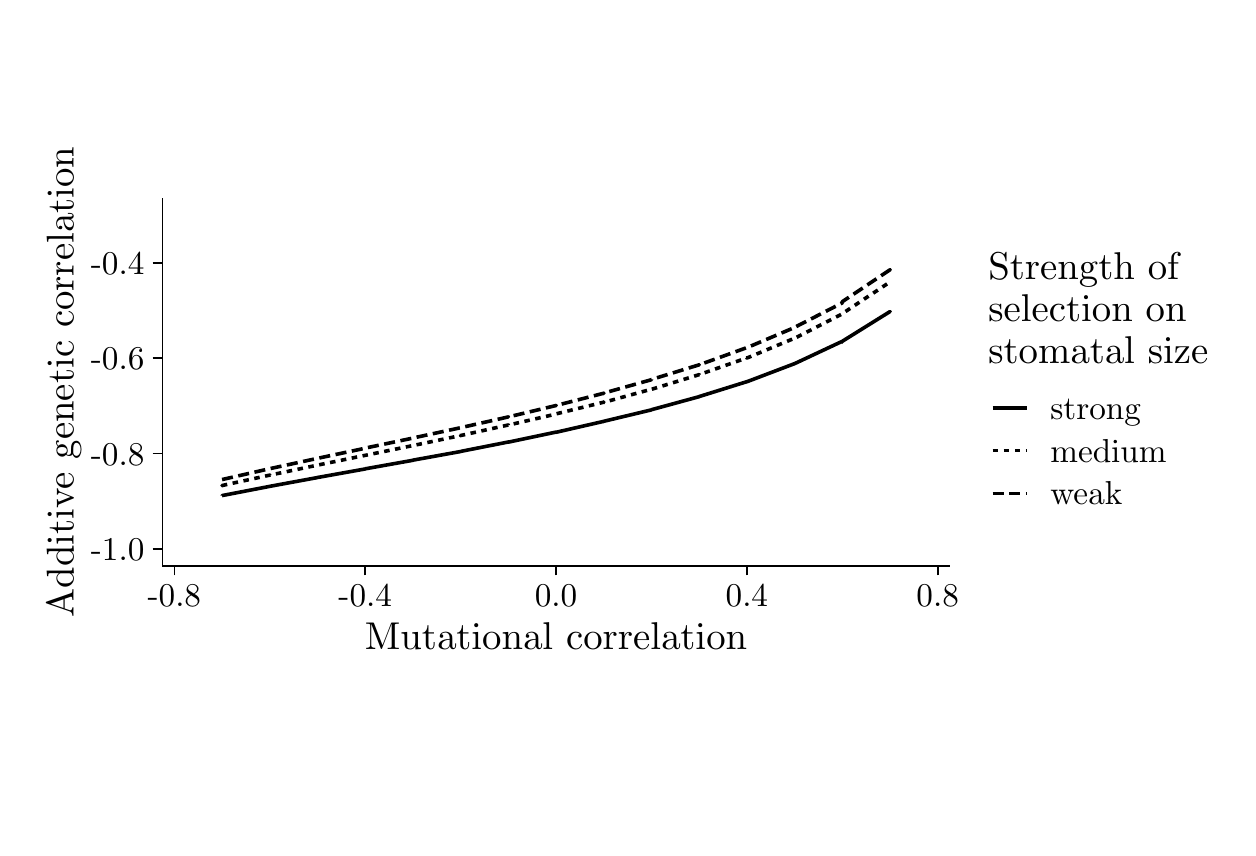
\begin{tikzpicture}[x=1pt,y=1pt]
\definecolor{fillColor}{RGB}{255,255,255}
\path[use as bounding box,fill=fillColor,fill opacity=0.00] (0,0) rectangle (433.62,289.08);
\begin{scope}
\path[clip] ( 48.69, 94.65) rectangle (333.15,227.39);
\definecolor{drawColor}{RGB}{0,0,0}

\path[draw=drawColor,line width= 1.3pt,line join=round] ( 70.24,119.98) --
	( 70.24,120.00) --
	( 87.48,123.33) --
	( 87.48,123.34) --
	(104.72,126.51) --
	(104.72,126.53) --
	(121.96,129.62) --
	(121.96,129.67) --
	(139.20,132.75) --
	(139.20,132.79) --
	(139.20,132.80) --
	(156.44,135.92) --
	(156.44,136.00) --
	(156.44,135.96) --
	(173.68,139.36) --
	(173.68,139.37) --
	(173.68,139.31) --
	(190.92,142.94) --
	(190.92,142.94) --
	(190.92,142.87) --
	(208.16,146.82) --
	(208.16,146.74) --
	(208.16,146.84) --
	(225.40,150.97) --
	(225.40,150.97) --
	(225.40,151.03) --
	(242.64,155.74) --
	(242.64,155.72) --
	(242.64,155.78) --
	(259.88,161.16) --
	(259.88,161.16) --
	(259.88,161.13) --
	(277.12,167.68) --
	(277.12,167.57) --
	(277.12,167.67) --
	(294.36,175.75) --
	(294.36,175.46) --
	(294.36,175.75) --
	(311.60,186.49) --
	(311.60,186.44) --
	(311.60,186.45);

\path[draw=drawColor,line width= 1.3pt,dash pattern=on 2pt off 2pt ,line join=round] ( 70.24,123.58) --
	( 70.24,123.56) --
	( 70.24,123.63) --
	( 87.48,127.39) --
	( 87.48,127.37) --
	( 87.48,127.37) --
	(104.72,131.00) --
	(104.72,131.00) --
	(104.72,131.00) --
	(121.96,134.54) --
	(121.96,134.55) --
	(121.96,134.53) --
	(139.20,138.08) --
	(139.20,138.11) --
	(139.20,138.07) --
	(156.44,141.70) --
	(156.44,141.72) --
	(156.44,141.70) --
	(173.68,145.51) --
	(173.68,145.49) --
	(173.68,145.47) --
	(190.92,149.45) --
	(190.92,149.46) --
	(190.92,149.52) --
	(208.16,153.74) --
	(208.16,153.83) --
	(208.16,153.69) --
	(225.40,158.44) --
	(225.40,158.52) --
	(225.40,158.39) --
	(242.64,163.70) --
	(242.64,163.70) --
	(242.64,163.69) --
	(259.88,169.76) --
	(259.88,169.74) --
	(259.88,169.69) --
	(277.12,176.87) --
	(277.12,176.94) --
	(277.12,176.81) --
	(294.36,185.67) --
	(294.36,185.68) --
	(294.36,185.74) --
	(311.60,197.19) --
	(311.60,197.16) --
	(311.60,197.23);

\path[draw=drawColor,line width= 1.3pt,dash pattern=on 4pt off 2pt ,line join=round] ( 70.24,125.79) --
	( 70.24,125.79) --
	( 87.48,129.72) --
	( 87.48,129.72) --
	(104.72,133.45) --
	(104.72,133.45) --
	(121.96,137.11) --
	(121.96,137.16) --
	(139.20,140.77) --
	(139.20,140.79) --
	(139.20,140.80) --
	(156.44,144.52) --
	(156.44,144.52) --
	(156.44,144.53) --
	(173.68,148.42) --
	(173.68,148.38) --
	(173.68,148.42) --
	(190.92,152.54) --
	(190.92,152.48) --
	(190.92,152.55) --
	(208.16,156.98) --
	(208.16,156.89) --
	(208.16,157.03) --
	(225.40,161.87) --
	(225.40,161.87) --
	(225.40,161.95) --
	(242.64,167.25) --
	(242.64,167.29) --
	(242.64,167.24) --
	(259.88,173.47) --
	(259.88,173.47) --
	(259.88,173.43) --
	(277.12,180.74) --
	(277.12,180.85) --
	(277.12,180.78) --
	(294.36,189.63) --
	(294.36,189.83) --
	(294.36,190.06) --
	(311.60,201.60) --
	(311.60,201.53) --
	(311.60,201.72);
\end{scope}
\begin{scope}
\path[clip] (  0.00,  0.00) rectangle (433.62,289.08);
\definecolor{drawColor}{RGB}{0,0,0}

\path[draw=drawColor,line width= 0.6pt,line join=round,line cap=rect] ( 48.69, 94.65) --
	( 48.69,227.39);
\end{scope}
\begin{scope}
\path[clip] (  0.00,  0.00) rectangle (433.62,289.08);
\definecolor{drawColor}{RGB}{0,0,0}

\node[text=drawColor,anchor=base east,inner sep=0pt, outer sep=0pt, scale=  1.20] at ( 42.19, 96.55) {-1.0};

\node[text=drawColor,anchor=base east,inner sep=0pt, outer sep=0pt, scale=  1.20] at ( 42.19,131.03) {-0.8};

\node[text=drawColor,anchor=base east,inner sep=0pt, outer sep=0pt, scale=  1.20] at ( 42.19,165.51) {-0.6};

\node[text=drawColor,anchor=base east,inner sep=0pt, outer sep=0pt, scale=  1.20] at ( 42.19,199.99) {-0.4};
\end{scope}
\begin{scope}
\path[clip] (  0.00,  0.00) rectangle (433.62,289.08);
\definecolor{drawColor}{RGB}{0,0,0}

\path[draw=drawColor,line width= 0.6pt,line join=round] ( 45.19,100.68) --
	( 48.69,100.68);

\path[draw=drawColor,line width= 0.6pt,line join=round] ( 45.19,135.16) --
	( 48.69,135.16);

\path[draw=drawColor,line width= 0.6pt,line join=round] ( 45.19,169.64) --
	( 48.69,169.64);

\path[draw=drawColor,line width= 0.6pt,line join=round] ( 45.19,204.12) --
	( 48.69,204.12);
\end{scope}
\begin{scope}
\path[clip] (  0.00,  0.00) rectangle (433.62,289.08);
\definecolor{drawColor}{RGB}{0,0,0}

\path[draw=drawColor,line width= 0.6pt,line join=round,line cap=rect] ( 48.69, 94.65) --
	(333.15, 94.65);
\end{scope}
\begin{scope}
\path[clip] (  0.00,  0.00) rectangle (433.62,289.08);
\definecolor{drawColor}{RGB}{0,0,0}

\path[draw=drawColor,line width= 0.6pt,line join=round] ( 53.00, 91.15) --
	( 53.00, 94.65);

\path[draw=drawColor,line width= 0.6pt,line join=round] (121.96, 91.15) --
	(121.96, 94.65);

\path[draw=drawColor,line width= 0.6pt,line join=round] (190.92, 91.15) --
	(190.92, 94.65);

\path[draw=drawColor,line width= 0.6pt,line join=round] (259.88, 91.15) --
	(259.88, 94.65);

\path[draw=drawColor,line width= 0.6pt,line join=round] (328.84, 91.15) --
	(328.84, 94.65);
\end{scope}
\begin{scope}
\path[clip] (  0.00,  0.00) rectangle (433.62,289.08);
\definecolor{drawColor}{RGB}{0,0,0}

\node[text=drawColor,anchor=base,inner sep=0pt, outer sep=0pt, scale=  1.20] at ( 53.00, 79.88) {-0.8};

\node[text=drawColor,anchor=base,inner sep=0pt, outer sep=0pt, scale=  1.20] at (121.96, 79.88) {-0.4};

\node[text=drawColor,anchor=base,inner sep=0pt, outer sep=0pt, scale=  1.20] at (190.92, 79.88) {0.0};

\node[text=drawColor,anchor=base,inner sep=0pt, outer sep=0pt, scale=  1.20] at (259.88, 79.88) {0.4};

\node[text=drawColor,anchor=base,inner sep=0pt, outer sep=0pt, scale=  1.20] at (328.84, 79.88) {0.8};
\end{scope}
\begin{scope}
\path[clip] (  0.00,  0.00) rectangle (433.62,289.08);
\definecolor{drawColor}{RGB}{0,0,0}

\node[text=drawColor,anchor=base,inner sep=0pt, outer sep=0pt, scale=  1.40] at (190.92, 64.41) {Mutational correlation};
\end{scope}
\begin{scope}
\path[clip] (  0.00,  0.00) rectangle (433.62,289.08);
\definecolor{drawColor}{RGB}{0,0,0}

\node[text=drawColor,rotate= 90.00,anchor=base,inner sep=0pt, outer sep=0pt, scale=  1.40] at ( 16.64,161.02) {Additive genetic correlation};
\end{scope}
\begin{scope}
\path[clip] (  0.00,  0.00) rectangle (433.62,289.08);
\definecolor{drawColor}{RGB}{0,0,0}

\node[text=drawColor,anchor=base west,inner sep=0pt, outer sep=0pt, scale=  1.40] at (347.15,197.92) {Strength of};

\node[text=drawColor,anchor=base west,inner sep=0pt, outer sep=0pt, scale=  1.40] at (347.15,182.80) {selection on};

\node[text=drawColor,anchor=base west,inner sep=0pt, outer sep=0pt, scale=  1.40] at (347.15,167.68) {stomatal size};
\end{scope}
\begin{scope}
\path[clip] (  0.00,  0.00) rectangle (433.62,289.08);
\definecolor{drawColor}{RGB}{0,0,0}

\path[draw=drawColor,line width= 1.3pt,line join=round] (348.69,151.62) -- (361.01,151.62);
\end{scope}
\begin{scope}
\path[clip] (  0.00,  0.00) rectangle (433.62,289.08);
\definecolor{drawColor}{RGB}{0,0,0}

\path[draw=drawColor,line width= 1.3pt,dash pattern=on 2pt off 2pt ,line join=round] (348.69,136.22) -- (361.01,136.22);
\end{scope}
\begin{scope}
\path[clip] (  0.00,  0.00) rectangle (433.62,289.08);
\definecolor{drawColor}{RGB}{0,0,0}

\path[draw=drawColor,line width= 1.3pt,dash pattern=on 4pt off 2pt ,line join=round] (348.69,120.82) -- (361.01,120.82);
\end{scope}
\begin{scope}
\path[clip] (  0.00,  0.00) rectangle (433.62,289.08);
\definecolor{drawColor}{RGB}{0,0,0}

\node[text=drawColor,anchor=base west,inner sep=0pt, outer sep=0pt, scale=  1.20] at (369.55,147.49) {strong};
\end{scope}
\begin{scope}
\path[clip] (  0.00,  0.00) rectangle (433.62,289.08);
\definecolor{drawColor}{RGB}{0,0,0}

\node[text=drawColor,anchor=base west,inner sep=0pt, outer sep=0pt, scale=  1.20] at (369.55,132.09) {medium};
\end{scope}
\begin{scope}
\path[clip] (  0.00,  0.00) rectangle (433.62,289.08);
\definecolor{drawColor}{RGB}{0,0,0}

\node[text=drawColor,anchor=base west,inner sep=0pt, outer sep=0pt, scale=  1.20] at (369.55,116.69) {weak};
\end{scope}
\end{tikzpicture}
